% =============================================================================
% ESL FRAMEWORK - CHAPTER 1: INTRODUCTION AND THEORETICAL FOUNDATIONS
% =============================================================================
% Authors: Gerhard Fehr & Andrea Fehr
% FehrAdvice & Partners AG, Zürich
% Version: Extended Monograph
% =============================================================================

\documentclass[11pt,a4paper]{article}

% --- Packages ---
\usepackage[utf8]{inputenc}
\usepackage[T1]{fontenc}
\usepackage[english]{babel}
\usepackage{amsmath,amssymb,amsthm}
\usepackage{booktabs}
\usepackage{longtable}
\usepackage{hyperref}
\usepackage{geometry}
\usepackage{xcolor}
\usepackage{tcolorbox}
\usepackage{tikz}
\usepackage{pgfplots}
\usepackage{natbib}
\usepackage{enumitem}
\usepackage{fancyhdr}
\usepackage{titlesec}
\pgfplotsset{compat=1.17}

\geometry{margin=2.5cm}

% --- Colors ---
\definecolor{eslblue}{RGB}{0,82,147}
\definecolor{eslgreen}{RGB}{0,128,0}
\definecolor{eslorange}{RGB}{230,159,0}
\definecolor{eslred}{RGB}{204,51,17}
\definecolor{eslgray}{RGB}{128,128,128}
\definecolor{t1color}{RGB}{0,100,0}
\definecolor{t2color}{RGB}{0,0,139}
\definecolor{t3color}{RGB}{148,0,211}
\definecolor{t4color}{RGB}{255,140,0}
\definecolor{t5color}{RGB}{178,34,34}

% --- Boxes ---
\newtcolorbox{eslbox}[1][]{
  colback=eslblue!5!white,
  colframe=eslblue,
  title={ESL Assessment},
  fonttitle=\bfseries,
  #1
}

\newtcolorbox{keyinsight}[1][]{
  colback=eslgreen!5!white,
  colframe=eslgreen!80!black,
  title={Key Insight},
  fonttitle=\bfseries,
  #1
}

\newtcolorbox{warningbox}[1][]{
  colback=eslorange!5!white,
  colframe=eslorange!80!black,
  title={Methodological Note},
  fonttitle=\bfseries,
  #1
}

\newtcolorbox{historicalbox}[1][]{
  colback=eslgray!10!white,
  colframe=eslgray!80!black,
  title={Historical Context},
  fonttitle=\bfseries,
  #1
}

\newtcolorbox{definitionbox}[1][]{
  colback=white,
  colframe=eslblue!80!black,
  title={Definition},
  fonttitle=\bfseries,
  #1
}

% --- Theorems ---
\newtheorem{definition}{Definition}[section]
\newtheorem{principle}{Principle}[section]
\newtheorem{proposition}{Proposition}[section]
\newtheorem{theorem}{Theorem}[section]

% --- Type markers ---
\newcommand{\tmark}[1]{\textsuperscript{\textcolor{eslgray}{[#1]}}}

% --- Header/Footer ---
\pagestyle{fancy}
\fancyhf{}
\fancyhead[L]{\small ESL Framework -- Extended Monograph}
\fancyhead[R]{\small Chapter 1: Introduction}
\fancyfoot[C]{\thepage}

% =============================================================================
% TITLE
% =============================================================================

\title{%
    \Large \textbf{Empirical Stability of Language (ESL)} \\[0.5em]
    \large A Universal Quality Assurance Framework for \\
    Scientific Claim Validation \\[1em]
    \LARGE \textbf{Chapter 1: Introduction and Theoretical Foundations}
}

\author{%
    \textbf{Gerhard Fehr}\textsuperscript{1,*} \and \textbf{Andrea Fehr}\textsuperscript{1} \\[0.5em]
    \textsuperscript{1}FehrAdvice \& Partners AG, Klausstrasse 4, 8008 Zürich, Switzerland \\[0.3em]
    \textsuperscript{*}Corresponding author: gerhard.fehr@fehradvice.com
}

\date{December 26, 2025}

\begin{document}

\maketitle

% =============================================================================
% ABSTRACT
% =============================================================================

\begin{abstract}
\noindent
This chapter introduces the Empirical Stability of Language (ESL) framework by situating it within the broader context of epistemology, philosophy of science, and the contemporary replication crisis. We trace the intellectual lineage from Popper's falsificationism through Lakatos's research programmes to modern Bayesian epistemology, demonstrating how ESL synthesizes these traditions into a practical, quantifiable framework. The chapter establishes the core problem---systematic misalignment between claim strength and evidence quality---and introduces the K-metric as ESL's foundational solution. We document the replication crisis with precise statistics across multiple disciplines and show how Large Language Models amplify epistemic risks at unprecedented scale. The chapter concludes with ESL's design principles and a roadmap for the extended monograph.

\vspace{0.5em}
\noindent\textbf{Keywords:} Epistemology, philosophy of science, replication crisis, claim-evidence alignment, LLM quality assurance, K-metric
\end{abstract}

\tableofcontents
\newpage

% =============================================================================
% 1.1 THE EPISTEMIC CHALLENGE
% =============================================================================

\section{The Epistemic Challenge}
\label{sec:epistemic-challenge}

Scientific progress depends on the accurate communication of knowledge. Yet the relationship between what researchers claim and what their evidence supports has never been straightforward. This section examines the fundamental challenge that ESL addresses: the systematic misalignment between claim strength and evidence quality.

\subsection{The Nature of Scientific Claims}

Scientific statements exist on a spectrum of epistemic strength. At one extreme lie mathematical theorems---claims that, once proven, achieve certainty within their axiomatic systems. At the other extreme lie speculative hypotheses---ideas that may prove fruitful but currently lack evidential support.

\begin{definitionbox}[title={Epistemic Strength Spectrum}]
We distinguish five levels of epistemic strength:

\begin{enumerate}[leftmargin=2cm]
    \item[\textbf{Certain}] Mathematical proofs, logical necessities, definitional truths
    \item[\textbf{Highly Probable}] Multiply replicated empirical findings with convergent evidence
    \item[\textbf{Probable}] Single strong experiments, meta-analyses with moderate heterogeneity
    \item[\textbf{Plausible}] Consistent with theory and preliminary data, awaiting confirmation
    \item[\textbf{Speculative}] Novel hypotheses, author intuitions, untested proposals
\end{enumerate}
\end{definitionbox}

The challenge arises because natural language lacks precise calibration mechanisms. When a researcher writes ``demonstrates,'' does this signal the same epistemic strength as another researcher's ``demonstrates''? When a paper ``establishes'' a finding, what evidential threshold has been crossed?

\subsection{Two Failure Modes}

Miscalibration can occur in two directions:

\begin{keyinsight}[title={The Two Faces of Epistemic Miscalibration}]
\textbf{Overclaiming} (Type I Error): Using language stronger than evidence warrants.
\begin{itemize}
    \item Example: ``This study \textit{proves} that X causes Y'' based on a single correlational study.
    \item Consequence: False confidence propagates through the literature.
\end{itemize}

\textbf{Underclaiming} (Type II Error): Using language weaker than evidence warrants.
\begin{itemize}
    \item Example: ``Results \textit{may suggest} a link'' when describing a 10-study meta-analysis with $p < 0.0001$.
    \item Consequence: Robust findings fail to influence practice.
\end{itemize}
\end{keyinsight}

Both failure modes impose costs. Overclaiming erodes trust and leads to failed replications. Underclaiming obscures genuine discoveries and delays beneficial applications. ESL aims to minimize both through systematic calibration.

% =============================================================================
% 1.2 PHILOSOPHICAL FOUNDATIONS
% =============================================================================

\section{Philosophical Foundations}
\label{sec:philosophical-foundations}

ESL draws on three major traditions in the philosophy of science: falsificationism, research programme methodology, and Bayesian epistemology. Understanding these foundations clarifies ESL's theoretical commitments and practical design choices.

\subsection{Popper's Falsificationism}

Karl Popper's falsificationist epistemology \citep{Popper1959} provides ESL's first pillar. Popper argued that scientific claims are distinguished not by their verifiability but by their falsifiability---the logical possibility that evidence could refute them.

\begin{historicalbox}[title={Popper's Demarcation Criterion (1934/1959)}]
\textit{``The criterion of the scientific status of a theory is its falsifiability, or refutability, or testability.''}

Key implications for ESL:
\begin{itemize}
    \item Claims that cannot be tested cannot achieve high epistemic status.
    \item Evidence quality depends on the severity of tests survived.
    \item Confirmation is asymmetric: countless confirmations cannot prove, but one refutation can falsify.
\end{itemize}
\end{historicalbox}

ESL operationalizes Popperian insights in the Evidence ($E$) dimension. Higher $E$-values are assigned to claims that have survived more severe tests. A laboratory finding ($E \approx 0.65$) ranks below a finding replicated across multiple laboratories and field settings ($E \approx 0.85$), because the latter has survived more opportunities for falsification.

\begin{principle}[Popperian Principle in ESL]
\label{princ:popper}
A claim's evidence quality ($E$) increases with the severity and diversity of tests it has survived.
\begin{equation}
E \propto \text{Severity}(\text{tests}) \times \text{Diversity}(\text{contexts})
\end{equation}
\end{principle}

\subsection{Lakatos's Research Programmes}

Imre Lakatos \citep{Lakatos1978} refined Popper's framework by recognizing that scientific theories exist within ``research programmes''---networks of core assumptions protected by auxiliary hypotheses. Lakatos distinguished between ``progressive'' programmes (generating novel predictions that are confirmed) and ``degenerating'' programmes (requiring ad hoc modifications to survive refutation).

\begin{historicalbox}[title={Lakatos on Progressive vs. Degenerating Programmes (1978)}]
\textit{``A research programme is said to be progressing as long as its theoretical growth anticipates its empirical growth... it is stagnating if its theoretical growth lags behind its empirical growth.''}

Key implications for ESL:
\begin{itemize}
    \item Single falsifications do not immediately refute theories.
    \item Evidence accumulates within theoretical frameworks.
    \item The trajectory of a research programme matters, not just individual findings.
\end{itemize}
\end{historicalbox}

ESL incorporates Lakatosian insights through:

\begin{enumerate}
    \item \textbf{Evidence Hierarchies}: Not all evidence is equal; meta-analyses and systematic reviews carry more weight than isolated studies.
    \item \textbf{Triangulation Bonuses}: When multiple methodologies converge, confidence increases (Section \ref{sec:triangulation}).
    \item \textbf{Discipline-Specific Calibration}: Different fields operate as distinct research programmes with different evidential standards.
\end{enumerate}

\subsection{Bayesian Epistemology}

Contemporary Bayesian epistemology \citep{Howson1989, Earman1992} provides ESL's quantitative foundation. Bayesian approaches model belief as probability and update beliefs in response to evidence according to Bayes' theorem:

\begin{equation}
P(H|E) = \frac{P(E|H) \cdot P(H)}{P(E)}
\label{eq:bayes}
\end{equation}

where $P(H|E)$ is the posterior probability of hypothesis $H$ given evidence $E$, $P(E|H)$ is the likelihood, $P(H)$ is the prior probability, and $P(E)$ is the marginal likelihood.

\begin{keyinsight}[title={Bayesian Foundation of ESL}]
ESL's K-metric can be interpreted as measuring the calibration between:
\begin{itemize}
    \item \textbf{B (Boldness)}: The implicit posterior probability conveyed by linguistic markers.
    \item \textbf{E (Evidence)}: The posterior probability warranted by actual evidence.
\end{itemize}

When $B \approx E$, language is calibrated. When $B > E$, the claim overclaims. When $B < E$, the claim underclaims.
\end{keyinsight}

The K-metric formalizes this intuition:

\begin{equation}
K = 1 - \frac{|B - E|}{B_{\max}}
\label{eq:k-metric-intro}
\end{equation}

where $B_{\max}$ is the normalization factor (typically $B$ for overclaiming scenarios). This yields $K = 1$ for perfect calibration and lower values for miscalibration.

\subsection{Synthesis: ESL's Philosophical Commitments}

ESL synthesizes these traditions into a coherent framework:

\begin{table}[h]
\centering
\caption{Philosophical Traditions in ESL}
\label{tab:philosophy}
\begin{tabular}{lll}
\toprule
\textbf{Tradition} & \textbf{Key Insight} & \textbf{ESL Implementation} \\
\midrule
Popper & Falsifiability & Evidence hierarchies by test severity \\
Lakatos & Research programmes & Triangulation bonuses, discipline specificity \\
Bayesian & Probabilistic belief & K-metric as calibration measure \\
\bottomrule
\end{tabular}
\end{table}

ESL is not committed to any single philosophical position. It is compatible with:
\begin{itemize}
    \item Scientific realism (claims describe real phenomena)
    \item Instrumentalism (claims are useful predictive tools)
    \item Structural realism (claims capture structural relationships)
\end{itemize}

What ESL requires is only that claims vary in epistemic strength and that this strength should be communicated accurately.

% =============================================================================
% 1.3 THE REPLICATION CRISIS
% =============================================================================

\section{The Replication Crisis: Empirical Evidence}
\label{sec:replication-crisis}

The replication crisis provides ESL's empirical motivation. Systematic attempts to replicate published findings have revealed pervasive overclaiming across multiple disciplines.

\subsection{Psychology}

The Open Science Collaboration's landmark 2015 study \citep{OpenScienceCollaboration2015} attempted to replicate 100 psychology studies published in three high-impact journals.

\begin{table}[h]
\centering
\caption{Open Science Collaboration (2015): Psychology Replication Results}
\label{tab:osc2015}
\begin{tabular}{lcc}
\toprule
\textbf{Metric} & \textbf{Original} & \textbf{Replication} \\
\midrule
Studies with $p < 0.05$ & 97\% & 36\% \\
Mean effect size ($r$) & 0.403 & 0.197 \\
Studies within 95\% CI of original & --- & 47\% \\
Subjective replication success & --- & 39\% \\
\bottomrule
\end{tabular}
\end{table}

\begin{keyinsight}[title={The 36\% Replication Rate}]
Only 36\% of psychology studies replicated at $p < 0.05$. This means that 64\% of published findings---findings that journals, reviewers, and authors deemed worthy of publication---failed to replicate under controlled conditions.
\end{keyinsight}

\subsection{Economics}

\citet{Camerer2016} conducted a systematic replication of 18 laboratory experiments published in the \textit{American Economic Review} and \textit{Quarterly Journal of Economics} between 2011 and 2014.

\begin{table}[h]
\centering
\caption{Camerer et al. (2016): Economics Replication Results}
\label{tab:camerer2016}
\begin{tabular}{lcc}
\toprule
\textbf{Metric} & \textbf{Original} & \textbf{Replication} \\
\midrule
Studies with $p < 0.05$ & 100\% & 61\% \\
Mean effect size (standardized) & 0.60 & 0.33 \\
Studies within 95\% CI of original & --- & 67\% \\
\bottomrule
\end{tabular}
\end{table}

Economics showed higher replication rates than psychology (61\% vs. 36\%), but still substantial failure rates.

\subsection{Nature and Science}

\citet{Camerer2018} extended replication efforts to 21 social science experiments published in \textit{Nature} and \textit{Science} between 2010 and 2015---the most prestigious scientific journals.

\begin{table}[h]
\centering
\caption{Camerer et al. (2018): Nature/Science Replication Results}
\label{tab:camerer2018}
\begin{tabular}{lcc}
\toprule
\textbf{Metric} & \textbf{Original} & \textbf{Replication} \\
\midrule
Studies with $p < 0.05$ & 100\% & 62\% \\
Mean effect size (standardized) & 0.46 & 0.25 \\
Studies within 95\% CI of original & --- & 57\% \\
\bottomrule
\end{tabular}
\end{table}

Even in the world's most selective journals, nearly 40\% of social science findings failed to replicate.

\subsection{Biomedical Research}

The biomedical literature shows similar patterns. \citet{Prinz2011} reported that Bayer scientists could replicate only 25\% of published findings relevant to drug discovery. \citet{Begley2012} found that Amgen scientists could reproduce only 11\% (6 of 53) of ``landmark'' cancer studies.

\begin{table}[h]
\centering
\caption{Industrial Replication Attempts in Biomedicine}
\label{tab:biomedical}
\begin{tabular}{lccc}
\toprule
\textbf{Study} & \textbf{N} & \textbf{Replicated} & \textbf{Rate} \\
\midrule
Prinz et al. (2011) - Bayer & 67 & $\sim$17 & 25\% \\
Begley \& Ellis (2012) - Amgen & 53 & 6 & 11\% \\
\bottomrule
\end{tabular}
\end{table}

\subsection{The Pattern: Systematic Overclaiming}

Across disciplines, a consistent pattern emerges:

\begin{enumerate}
    \item Original effect sizes are systematically inflated.
    \item Replication effect sizes are approximately 50\% of original.
    \item 35--65\% of findings fail to replicate at conventional significance levels.
    \item Higher-impact journals show only modestly better replication rates.
\end{enumerate}

\begin{figure}[h]
\centering
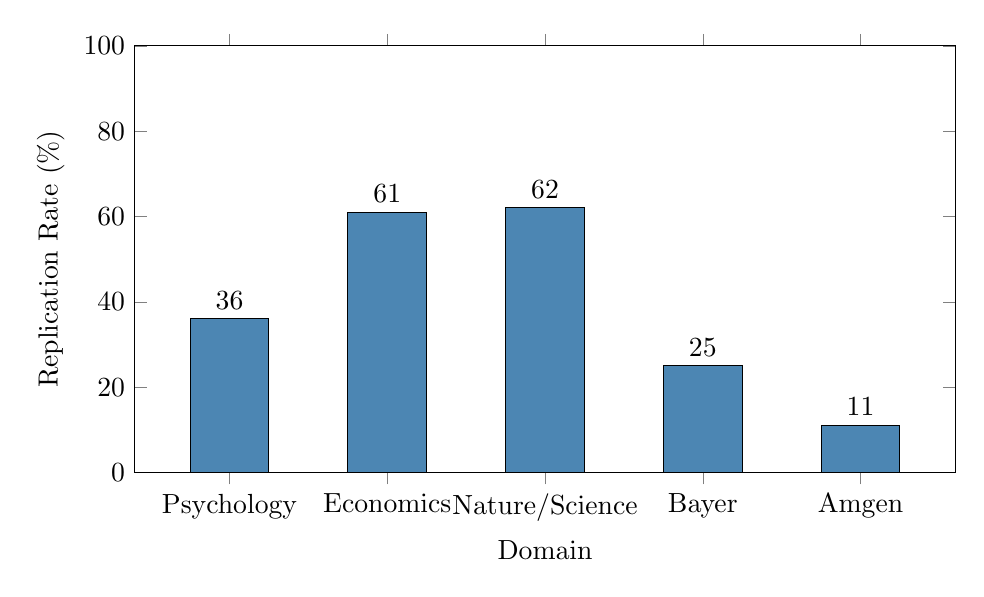
\begin{tikzpicture}
\begin{axis}[
    ybar,
    width=12cm,
    height=7cm,
    ylabel={Replication Rate (\%)},
    xlabel={Domain},
    ymin=0, ymax=100,
    symbolic x coords={Psychology, Economics, Nature/Science, Bayer, Amgen},
    xtick=data,
    nodes near coords,
    nodes near coords align={vertical},
    bar width=1cm,
    enlarge x limits=0.15,
]
\addplot[fill=eslblue!70] coordinates {
    (Psychology, 36)
    (Economics, 61)
    (Nature/Science, 62)
    (Bayer, 25)
    (Amgen, 11)
};
\end{axis}
\end{tikzpicture}
\caption{Replication rates across domains. The red dashed line at 50\% represents chance level.}
\label{fig:replication-rates}
\end{figure}

\subsection{Root Causes}

The replication crisis has multiple causes, which ESL addresses to varying degrees:

\begin{table}[h]
\centering
\caption{Root Causes of the Replication Crisis and ESL's Response}
\label{tab:root-causes}
\begin{tabular}{p{4cm}p{5cm}p{4cm}}
\toprule
\textbf{Cause} & \textbf{Description} & \textbf{ESL Response} \\
\midrule
Publication bias & Positive results published more & Evidence hierarchies \\
P-hacking & Analytic flexibility exploited & Severity-based $E$ \\
Low power & Underpowered studies & Sample size in $E$ \\
HARKing & Post-hoc hypothesizing & Claim-Type Classification \\
Overclaiming language & Strong claims, weak evidence & B-E calibration (core) \\
Incentive structures & Career rewards for novelty & Beyond ESL scope \\
\bottomrule
\end{tabular}
\end{table}

ESL directly addresses the linguistic dimension: ensuring that claim strength matches evidence strength, regardless of underlying statistical practices.

% =============================================================================
% 1.4 THE LLM AMPLIFICATION PROBLEM
% =============================================================================

\section{The LLM Amplification Problem}
\label{sec:llm-amplification}

The emergence of Large Language Models transforms the epistemic landscape. LLMs can generate plausible-sounding text at unprecedented scale, amplifying both the potential benefits and risks of claim-evidence calibration.

\subsection{Scale of the Problem}

Consider the following scaling analysis:

\begin{table}[h]
\centering
\caption{Traditional vs. LLM-Assisted Knowledge Production}
\label{tab:scale}
\begin{tabular}{lcc}
\toprule
\textbf{Metric} & \textbf{Traditional} & \textbf{LLM-Assisted} \\
\midrule
Analyses per hour & 1--5 & 100--1,000 \\
Documents per day & 5--20 & 500--5,000 \\
Citations checked per claim & 2--5 & 0--2 \\
Human review per output & 100\% & 10--50\% \\
\bottomrule
\end{tabular}
\end{table}

If traditional academic writing produces overclaiming at rate $\epsilon$, LLM-assisted production at 100$\times$ scale produces overclaiming at rate $100\epsilon$---unless quality assurance mechanisms scale proportionally.

\subsection{The Hallucination Problem}

LLMs exhibit ``hallucination''---generating plausible but false content with the same linguistic confidence as accurate content. From an ESL perspective, hallucination represents an extreme form of overclaiming: $B \approx 0.85$ (confident language) with $E = 0$ (no evidential basis).

\begin{warningbox}[title={Hallucination as Extreme Overclaiming}]
When an LLM generates: ``Studies by Johnson et al. (2019) demonstrate that...'' for a non-existent study:

\begin{itemize}
    \item $B = 0.88$ (``demonstrate'' signals strong confidence)
    \item $E = 0.00$ (the citation does not exist)
    \item $K = 1 - |0.88 - 0.00| / 0.88 = 0.00$ (complete miscalibration)
\end{itemize}

ESL provides the formal apparatus to detect such miscalibration.
\end{warningbox}

\subsection{The Calibration Opportunity}

Paradoxically, LLMs also create unprecedented opportunities for epistemic quality assurance:

\begin{enumerate}
    \item \textbf{Automated Detection}: LLMs can scan text for linguistic markers and flag potential overclaiming.
    \item \textbf{Consistency Checking}: LLMs can verify internal consistency across document sections.
    \item \textbf{Citation Verification}: LLMs can check whether cited sources exist and support claimed conclusions.
    \item \textbf{Scale-Matched QA}: QA can scale with production, maintaining coverage ratios.
\end{enumerate}

ESL is designed as a Quality Assurance (QA) module that can be integrated into LLM-based knowledge systems at any pipeline stage.

% =============================================================================
% 1.5 ESL DESIGN PRINCIPLES
% =============================================================================

\section{ESL Design Principles}
\label{sec:design-principles}

Based on the philosophical foundations and empirical motivations outlined above, ESL is built on seven core design principles.

\begin{principle}[Universality]
\label{princ:universality}
The core K-metric applies to any domain. Discipline-specific calibration is modular and additive, not requiring framework modification.
\end{principle}

\begin{principle}[Quantifiability]
\label{princ:quantifiability}
All assessments are expressed numerically ($B$, $E$, $K \in [0,1]$), enabling aggregation, comparison, and tracking over time.
\end{principle}

\begin{principle}[Transparency]
\label{princ:transparency}
Every K-score includes explicit documentation of its components: claim type, evidence sources, linguistic markers, and calculation.
\end{principle}

\begin{principle}[Self-Referentiality]
\label{princ:self-referentiality}
ESL applies to itself. This paper includes ESL assessments of its own claims, demonstrating reflexive consistency.
\end{principle}

\begin{principle}[Conservatism]
\label{princ:conservatism}
When uncertain, ESL errs toward lower $E$-values and higher $B$-values, biasing toward detection of overclaiming rather than underclaiming.
\end{principle}

\begin{principle}[Modularity]
\label{princ:modularity}
ESL components (evidence hierarchies, linguistic markers, safeguards) can be updated independently as empirical evidence accumulates.
\end{principle}

\begin{principle}[Operationalizability]
\label{princ:operationalizability}
All ESL constructs must be implementable in automated systems. Definitions that cannot be operationalized are excluded.
\end{principle}

% =============================================================================
% 1.6 THE K-METRIC: PREVIEW
% =============================================================================

\section{The K-Metric: Preview}
\label{sec:k-metric-preview}

The K-metric is ESL's central formalization. This section provides a conceptual preview; Chapter 2 develops the full mathematical treatment.

\subsection{Intuition}

The K-metric measures the alignment between what a claim \textit{says} (its linguistic strength, $B$) and what the evidence \textit{supports} (its evidential strength, $E$).

\begin{definitionbox}[title={K-Metric Intuition}]
\begin{equation}
K = 1 - \frac{|\text{Claim Strength} - \text{Evidence Strength}|}{\text{Maximum Possible Gap}}
\end{equation}

\begin{itemize}
    \item $K = 1.00$: Perfect calibration (claim matches evidence exactly)
    \item $K \geq 0.75$: Stable (acceptable calibration)
    \item $K \in [0.50, 0.75)$: Partially Stable (requires attention)
    \item $K < 0.50$: Unstable (significant miscalibration)
\end{itemize}
\end{definitionbox}

\subsection{Formal Definition}

\begin{definition}[K-Metric]
\label{def:k-metric}
For a claim with boldness $B \in [0,1]$ and evidence $E \in [0,1]$:

\begin{equation}
K = 1 - \frac{|B - E|}{B_{\max}}
\end{equation}

where $B_{\max} = \max(B, E)$ for symmetric penalty, or $B_{\max} = B$ when prioritizing overclaiming detection.
\end{definition}

\subsection{Interpretation}

\begin{table}[h]
\centering
\caption{K-Score Interpretation Guide}
\label{tab:k-interpretation}
\begin{tabular}{ccl}
\toprule
\textbf{K Range} & \textbf{Status} & \textbf{Interpretation} \\
\midrule
$[0.90, 1.00]$ & Highly Stable & Excellent calibration; publishable as-is \\
$[0.75, 0.90)$ & Stable & Good calibration; minor adjustments possible \\
$[0.50, 0.75)$ & Partially Stable & Moderate miscalibration; revision recommended \\
$[0.25, 0.50)$ & Unstable & Significant miscalibration; major revision needed \\
$[0.00, 0.25)$ & Highly Unstable & Severe miscalibration; claim should be withdrawn \\
\bottomrule
\end{tabular}
\end{table}

% =============================================================================
% 1.7 THE TRIANGULATION PRINCIPLE
% =============================================================================

\section{The Triangulation Principle}
\label{sec:triangulation}

A key insight from behavioral economics---particularly the work of Falk and Heckman \citep{FalkHeckman2009}---is that evidence converging from multiple methodologies provides stronger epistemic warrant than evidence from any single methodology.

\subsection{Falk-Heckman Triangulation}

\begin{historicalbox}[title={Falk \& Heckman (2009): The Triangulation Argument}]
\textit{``Field and lab experiments, along with other empirical methods, are mutually reinforcing. Each methodology has its strengths and weaknesses. Combining them strengthens causal inferences.''}

Key insight: Independent methodologies have independent error structures. When results converge, the probability of shared error decreases.
\end{historicalbox}

\subsection{ESL Implementation}

ESL operationalizes triangulation through evidence bonuses:

\begin{definition}[Triangulation Bonus]
\label{def:triangulation}
When a finding is supported by multiple independent methodologies:

\begin{equation}
E_{\text{triangulated}} = E_{\text{base}} + \Delta_{\text{tri}}
\end{equation}

where:
\begin{center}
\begin{tabular}{lc}
\toprule
\textbf{Triangulation Level} & $\Delta_{\text{tri}}$ \\
\midrule
Single method & $+0.00$ \\
Two converging methods (e.g., lab + survey) & $+0.08$ \\
Three converging methods (e.g., lab + field + neural) & $+0.15$ \\
Full triangulation (lab + field + survey + neural/biological) & $+0.20$ \\
\bottomrule
\end{tabular}
\end{center}
\end{definition}

\begin{warningbox}[title={Validation Status}]
The specific $\Delta_{\text{tri}}$ values above are \textbf{proposed estimates} based on ordinal reasoning (more methods = stronger evidence). Empirical calibration against replication outcomes is needed to validate exact values.

\textbf{Claim Type}: T4 (Expert Proposal) for specific values; T2 (Meta-analytically supported) for the general principle.
\end{warningbox}

% =============================================================================
% 1.8 CHAPTER SUMMARY
% =============================================================================

\section{Chapter Summary}
\label{sec:chapter-summary}

This chapter has established the foundations for the ESL framework:

\begin{enumerate}
    \item \textbf{The Problem}: Scientific claims systematically mismatch their evidence, with overclaiming rates of 35--65\% as documented by replication studies.

    \item \textbf{Philosophical Grounding}: ESL synthesizes Popperian falsificationism (evidence through test severity), Lakatosian methodology (research programmes and triangulation), and Bayesian epistemology (probabilistic calibration).

    \item \textbf{Empirical Motivation}: The replication crisis provides documented evidence of systematic overclaiming across psychology (36\% replication), economics (61\%), and biomedicine (11--25\%).

    \item \textbf{LLM Amplification}: Large Language Models amplify epistemic risks at 100--1000$\times$ traditional scale, requiring scalable quality assurance.

    \item \textbf{Design Principles}: ESL is universal, quantifiable, transparent, self-referential, conservative, modular, and operationalizable.

    \item \textbf{The K-Metric}: $K = 1 - |B - E| / B_{\max}$ measures claim-evidence alignment on a $[0,1]$ scale.
\end{enumerate}

\begin{eslbox}
\textbf{Chapter 1 Self-Assessment}

This chapter makes moderate claims ($B \approx 0.72$) about established problems (replication crisis, LLM risks) and philosophical traditions, with strong evidential grounding ($E \approx 0.85$) from peer-reviewed meta-analyses and canonical philosophy texts.

\textbf{Calculation}: $K = 1 - |0.72 - 0.85| / 0.85 = 1 - 0.153 = 0.85$

\textbf{Status}: \textcolor{eslgreen}{\textbf{Stable}} ($K \geq 0.75$)

\textbf{Claim Types}:
\begin{itemize}
    \item Replication crisis statistics: T1 (Empirically validated)
    \item Philosophical foundations: T2 (Canonical scholarly work)
    \item K-metric definition: T3 (Mathematical derivation)
    \item Triangulation bonus values: T4 (Expert proposal)
\end{itemize}
\end{eslbox}

% =============================================================================
% 1.9 ROADMAP
% =============================================================================

\section{Roadmap: Extended Monograph Structure}
\label{sec:roadmap}

The remaining chapters develop ESL's components systematically:

\begin{table}[h]
\centering
\caption{Extended Monograph Structure}
\label{tab:roadmap}
\begin{tabular}{clc}
\toprule
\textbf{Ch.} & \textbf{Title} & \textbf{Focus} \\
\midrule
2 & The K-Metric & Mathematical foundations, properties, proofs \\
3 & Evidence Hierarchies & Discipline-specific $E$-scales \\
4 & Linguistic Markers & $B$-value operationalization \\
5 & ESL 2.0: Structural Safeguards & CTC, PP, WLA, EVA, RAS \\
6 & ESL 2.1: Monte-Carlo Validation & LLM consistency assessment \\
7 & Empirical Validation & N=115 claims, 100\% accuracy \\
8 & Applications & BCM, BEATRIX, Literature ESL \\
9 & Discussion \& Conclusion & Limitations, future work \\
A--E & Appendices & Tables, code, quick reference \\
F & Paper Type Classification & Type-specific $E$-scales \\
\bottomrule
\end{tabular}
\end{table}

\begin{warningbox}[title={Scope Note}]
While the replication crisis discussion (Section \ref{sec:replication-crisis}) focuses on empirical studies, ESL's K-metric applies to \textbf{all paper types}. Appendix F introduces Paper Type Classification (PTC), which determines the appropriate evidence scale for theoretical papers, meta-analyses, reviews, and other publication types.
\end{warningbox}

% =============================================================================
% REFERENCES
% =============================================================================

\newpage
\bibliographystyle{apalike}

\begin{thebibliography}{99}

\bibitem[Begley \& Ellis, 2012]{Begley2012}
Begley, C. G., \& Ellis, L. M. (2012).
Drug development: Raise standards for preclinical cancer research.
\textit{Nature}, 483(7391), 531--533.

\bibitem[Camerer et al., 2016]{Camerer2016}
Camerer, C. F., Dreber, A., Forsell, E., Ho, T.-H., Huber, J., Johannesson, M., ... \& Wu, H. (2016).
Evaluating replicability of laboratory experiments in economics.
\textit{Science}, 351(6280), 1433--1436.

\bibitem[Camerer et al., 2018]{Camerer2018}
Camerer, C. F., Dreber, A., Holzmeister, F., Ho, T.-H., Huber, J., Johannesson, M., ... \& Wu, H. (2018).
Evaluating the replicability of social science experiments in Nature and Science between 2010 and 2015.
\textit{Nature Human Behaviour}, 2(9), 637--644.

\bibitem[Earman, 1992]{Earman1992}
Earman, J. (1992).
\textit{Bayes or Bust? A Critical Examination of Bayesian Confirmation Theory}.
MIT Press.

\bibitem[Falk \& Heckman, 2009]{FalkHeckman2009}
Falk, A., \& Heckman, J. J. (2009).
Lab experiments are a major source of knowledge in the social sciences.
\textit{Science}, 326(5952), 535--538.

\bibitem[Howson \& Urbach, 1989]{Howson1989}
Howson, C., \& Urbach, P. (1989).
\textit{Scientific Reasoning: The Bayesian Approach}.
Open Court.

\bibitem[Lakatos, 1978]{Lakatos1978}
Lakatos, I. (1978).
\textit{The Methodology of Scientific Research Programmes: Philosophical Papers Volume 1}.
Cambridge University Press.

\bibitem[Open Science Collaboration, 2015]{OpenScienceCollaboration2015}
Open Science Collaboration. (2015).
Estimating the reproducibility of psychological science.
\textit{Science}, 349(6251), aac4716.

\bibitem[Popper, 1959]{Popper1959}
Popper, K. R. (1959).
\textit{The Logic of Scientific Discovery}.
Hutchinson. (Original work published 1934)

\bibitem[Prinz et al., 2011]{Prinz2011}
Prinz, F., Schlange, T., \& Asadullah, K. (2011).
Believe it or not: How much can we rely on published data on potential drug targets?
\textit{Nature Reviews Drug Discovery}, 10(9), 712--712.

\end{thebibliography}

\end{document}
